\section{Rebasing}
Suppose that you create a branch "mywork" on a remote-tracking branch "origin".
\lstset{basicstyle=\scriptsize, numbers=none, captionpos=b, tabsize=4}
\begin{lstlisting}[caption=,language={bash},
breaklines=true,label=lst:]
$ git checkout -b mywork origin
\end{lstlisting}

\begin{figure}[h]
\centering
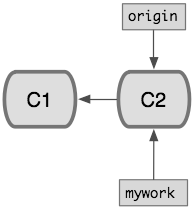
\includegraphics[width=0.20\textwidth]{content/git/rebase0.png}
\end{figure}

Now you do some work, creating two new commits.
\lstset{basicstyle=\scriptsize, numbers=none, captionpos=b, tabsize=4}
\begin{lstlisting}[caption=,language={bash},
breaklines=true,label=lst:]
$ vi file.txt
$ git commit
$ vi otherfile.txt
$ git commit
...
\end{lstlisting}

Meanwhile, someone else does some work creating two new commits on the origin
branch too. This means both 'origin' and 'mywork' has advanced, which means the
work has diverged.

\begin{figure}[h]
\centering
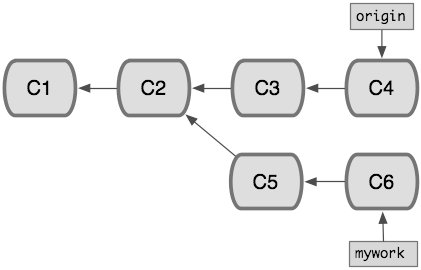
\includegraphics[width=0.43\textwidth]{content/git/rebase1.png}
\end{figure}

At this point, you could use "pull" to merge your changes back in; the result
would create a new merge commit, like this:

\begin{figure}[h]
\centering
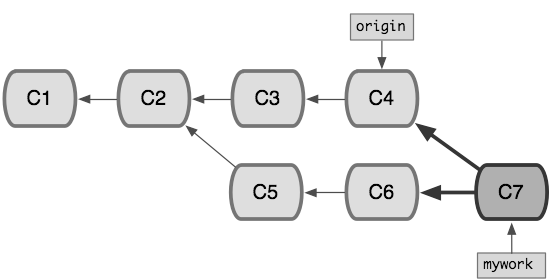
\includegraphics[width=0.43\textwidth]{content/git/rebase2.png}
\end{figure}

However, if you prefer to keep the history in mywork a simple series of commits
without any merges, you may instead choose to use git rebase:

\section{git merge}
\begin{figure}[h]
\centering
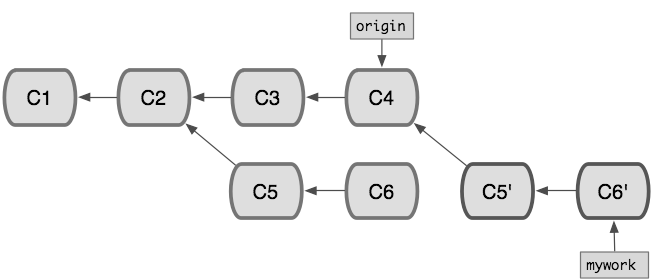
\includegraphics[width=0.43\textwidth]{content/git/rebase3.png}
\end{figure}

\lstset{basicstyle=\scriptsize, numbers=none, captionpos=b, tabsize=4}
\begin{lstlisting}[caption=,language={bash},
breaklines=true,label=lst:]
$ git checkout mywork
$ git rebase origin
\end{lstlisting}

This will remove each of your commits from mywork, temporarily saving them as
patches (in a directory named ".git/rebase"), update mywork to point at the
latest version of origin, then apply each of the saved patches to the new
mywork.

Once the ref ('mywork') is updated to point to the newly created commit
objects, your older commits will be abandoned. They will likely be removed if
you run a pruning garbage collection. (see git gc)
\begin{figure}[h]
\centering
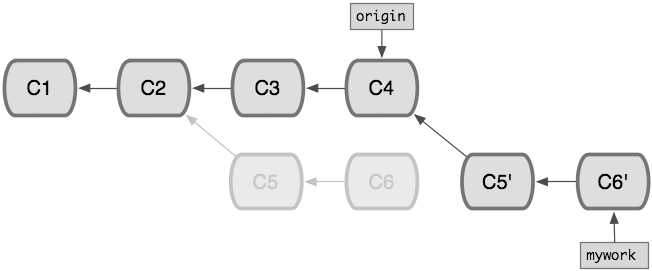
\includegraphics[width=0.43\textwidth]{content/git/rebase4.png}
\end{figure}

So now we can look at the difference in our history between running a merge and
running a rebase:
\begin{figure}[h]
\centering
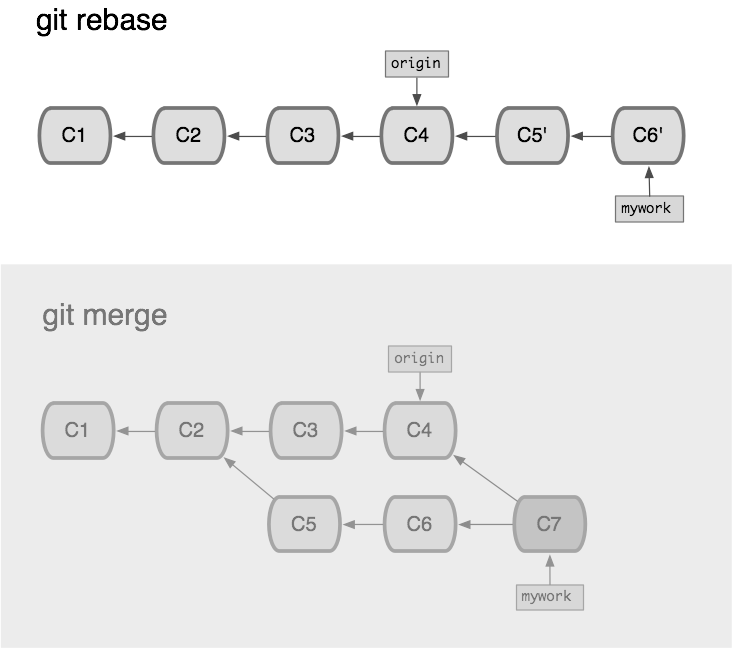
\includegraphics[width=0.43\textwidth]{content/git/rebase5.png}
\end{figure}


In the process of the rebase, it may discover conflicts. In that case it will
stop and allow you to fix the conflicts; after fixing conflicts, use "git-add"
to update the index with those contents, and then, instead of running
git-commit, just run
\lstset{basicstyle=\scriptsize, numbers=none, captionpos=b, tabsize=4}
\begin{lstlisting}[caption=,language={bash},
breaklines=true,label=lst:]
$ git rebase --continue
\end{lstlisting}

and git will continue applying the rest of the patches.

At any point you may use the --abort option to abort this process and return
mywork to the state it had before you started the rebase:

\lstset{basicstyle=\scriptsize, numbers=none, captionpos=b, tabsize=4}
\begin{lstlisting}[caption=,language={bash},
breaklines=true,label=lst:]
$ git rebase --abort
\end{lstlisting}
